
\subsection{Group 4 - Supply Chain Standalone Points of Improvement and Blockchain+SC points of Applicability and Improvement}

%Problema: há varios graficos para mostrar, mas alguns deles, como o da figura 6.1, têm varias (7 a 8) distribuições para mostrar, onde cada uma delas tem os seus valores das metricas.

%2 EM 1
%GRAFICOS DOS SUPPLY CHAIN IMPROVEMENT ASPECTS

%TODO: VALE A PENA DIVIDIR EM VARIAS IMAGENS?

\subsection*{1 - Rank the importance of some aspects which Supply Chains aim to improve.}
 
(Placeholder image. Should i divide it in more images?)

\begin{figure}[h]
\centering
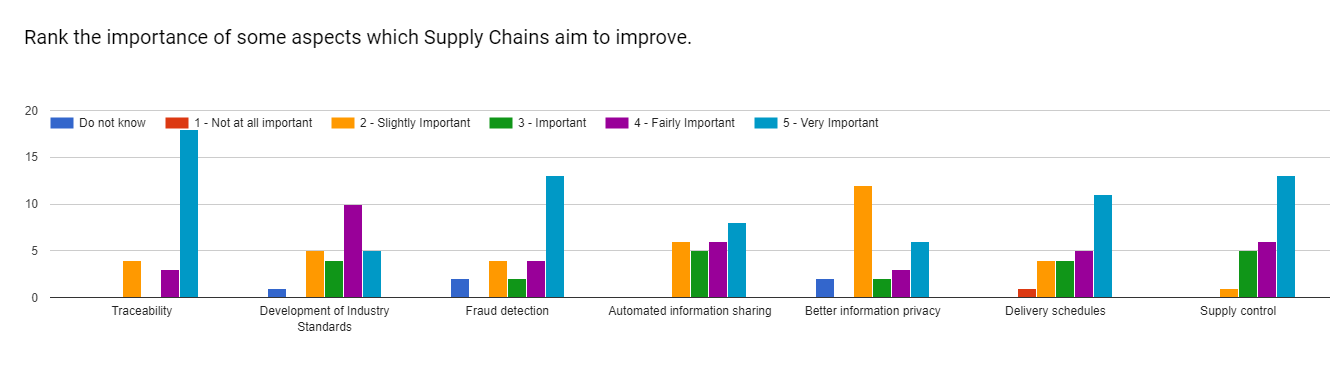
\includegraphics[scale=0.35]{media/importance_SC_improvement_points.png}
\caption["Rank the importance of some aspects which Supply Chains aim to improve."]{"Rank the importance of some aspects which Supply Chains aim to improve."}
\label{fig:importance_SC_improvement_points}
\end{figure}

%%%%%%%% TABLE BEGIN %%%%%%%%%

\begin{table}[h]
\centering

\begin{tabular}{l|l|l|l|l|l|l|}
\cline{2-7}
                                                                                                    & Mode & Median & Mean   & \begin{tabular}[c]{@{}l@{}}Standard\\ Deviation\end{tabular} & Range & Skewness \\ \hline
\multicolumn{1}{|l|}{Traceability}                                                                  & 5    & 5      & 4,400  & 1,1180                                                       & 3     & -1,6722  \\ \hline
\multicolumn{1}{|l|}{\begin{tabular}[c]{@{}l@{}}Development\\ of Industry\\ Standards\end{tabular}} & 4    & 4      & 3,6250 & 1,0555                                                       & 3     & -0,3592  \\ \hline
\multicolumn{1}{|l|}{\begin{tabular}[c]{@{}l@{}}Fraud\\ Detection\end{tabular}}                     & 5    & 5      & 4,1304 & 1,1795                                                       & 3     & -1,0019  \\ \hline
\multicolumn{1}{|l|}{\begin{tabular}[c]{@{}l@{}}Automated\\ Information \\ Sharing\end{tabular}}    & 5    & 4      & 3,6400 & 1,1860                                                       & 3     & -0,2001  \\ \hline
\multicolumn{1}{|l|}{\begin{tabular}[c]{@{}l@{}}Better\\ Information\\ privacy\end{tabular}}        & 2    & 2      & 3,1304 & 1,3247                                                       & 3     & 0,5105   \\ \hline
\multicolumn{1}{|l|}{\begin{tabular}[c]{@{}l@{}}Delivery\\ Schedules\end{tabular}}                  & 5    & 4      & 3,8400 & 1,2806                                                       & 4     & -0,7117  \\ \hline
\multicolumn{1}{|l|}{Supply Control}                                                                & 5    & 5      & 4,2400 & 0,9256                                                       & 3     & -0,8653  \\ \hline
\end{tabular}
\caption{My caption}
\label{my-label}
\end{table}

%%%%%%%% TABLE END %%%%%%%%%%%%%%%%

\begin{enumerate}
    \item Traceability - Give explanation about how important Traceability is, taking into account these values; informal explanation that it is a really high agreement, since the mode and median are both 5; not only is it the most popular choice, but it was also chosen by 50\% of the people. At the same time, the mean shows us that average popularity is 4.4. The answer has a range of 3, with the values 2 through 5 being selected as the extremes. This means there was either someone dissatisfied, or they had a bad day; etc etc, give more explanations? Or is this ok?
    \item Development of Industry Standards - REPEAT AS ABOVE
    \item Fraud Detection
    \item Automated Information Sharing
    \item Better Information Privacy
    \item Delivery Schedules
    \item Supply Control
\end{enumerate}
    
    All 7 improvement aspects where studied: rank them by the 3 with highest mean? Highest median? Combination of both (how to combine?)  ?

%2 EM 1https://www.overleaf.com/13104200fnmytzmhwtck#
%GRAFICOS DOS BLOCKCHAIN POINTS OF APPLICABILITY
\subsection*{2 - Rank the importance of the following functionalities for an information system that stores or processes data pertaining to a Supply Chain}

\begin{figure}[h]
\centering
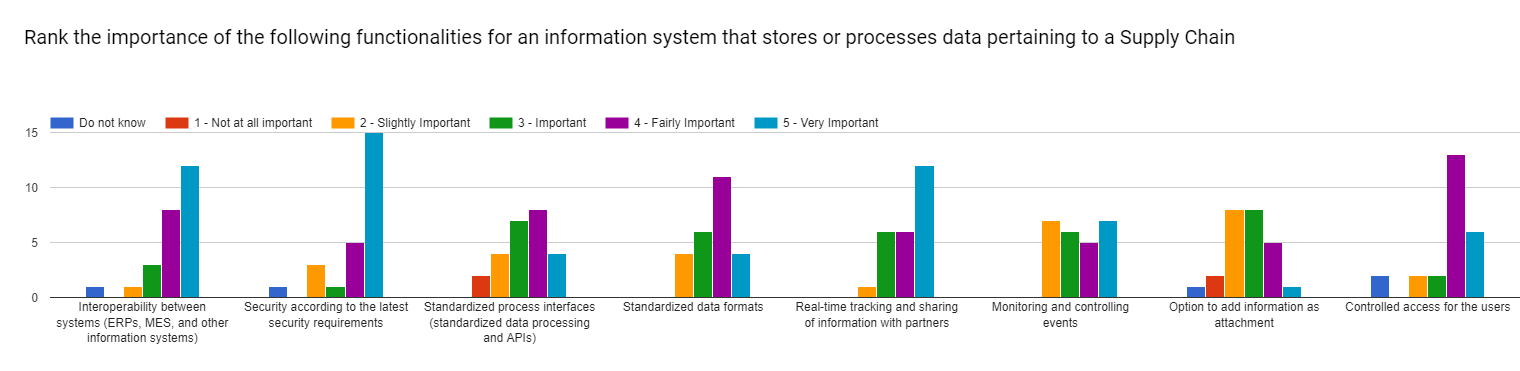
\includegraphics[scale=0.28]{media/importance_SC_info_systems.png}
\caption["Rank the importance of some functionalities in a supply chain based information system."]{"Rank the importance of some functionalities in a supply chain based information system."}
\label{fig:importance_SC_info_systems}
\end{figure}

%%%% TABLE START %%%%%%%%%%

\begin{table}[h]
\centering
\caption{My caption}
\label{my-label}
\begin{tabular}{l|c|c|c|c|c|c|}
\cline{2-7}
                                                                                                                                                & \multicolumn{1}{l|}{Mode} & \multicolumn{1}{l|}{Median} & \multicolumn{1}{l|}{Mean} & \multicolumn{1}{l|}{\begin{tabular}[c]{@{}l@{}}Standard\\  Deviation\end{tabular}} & \multicolumn{1}{l|}{Range} & \multicolumn{1}{l|}{Skewness} \\ \hline
\multicolumn{1}{|l|}{\begin{tabular}[c]{@{}l@{}}Interoperability Between \\ Systems (ERPs, MES, \\ and other information systems)\end{tabular}} & 5                         & 4,5                         & 4,2917                    & 0,8587                                                                             & 3                          & -1,0813                       \\ \hline
\multicolumn{1}{|l|}{\begin{tabular}[c]{@{}l@{}}Development of Industry\\ Standards\end{tabular}}                                               & 5                         & 5                           & 4,3333                    & 1,0495                                                                             & 3                          & -1,4862                       \\ \hline
\multicolumn{1}{|l|}{\begin{tabular}[c]{@{}l@{}}Standardized Process Interfaces \\ (Data Processing and APIs)\end{tabular}}                     & 4                         & 3                           & 3,3200                    & 1,1804                                                                             & 3                          & -0,3558                       \\ \hline
\multicolumn{1}{|l|}{Standardized Data Formats}                                                                                                 & 4                         & 4                           & 3,6000                    & 0,9574                                                                             & 3                          & -0,3096                       \\ \hline
\multicolumn{1}{|l|}{\begin{tabular}[c]{@{}l@{}}Real-time tracking and sharing \\ of information with partners\end{tabular}}                    & 5                         & 4                           & 4,1600                    & 0,9434                                                                             & 3                          & -0,6664                       \\ \hline
\multicolumn{1}{|l|}{Monitoring and controlling events}                                                                                         & 5                         & 3                           & 3,4800                    & 1,1944                                                                             & 3                          & 0,0513                       \\ \hline
\multicolumn{1}{|l|}{\begin{tabular}[c]{@{}l@{}}Option to add information \\ as attachment\end{tabular}}                                        & 2                         & 3                           & 2,7917                    & 1,0206                                                                             & 4                          & 0,1870                        \\ \hline
\multicolumn{1}{|l|}{Controlled access for the users}                                                                                           & 4                         & 4                           & 4                         & 0,8528                                                                             & 3                          & -0,9632                       \\ \hline
\end{tabular}
\end{table}

%%%% TABLE END %%%%%%%%%%

%GRAFICO DA ULTIMA PERGUNTA DE RATE THE AFFIRMATION, A VER COM BLOCKCHAIN E INFORMATION SYSTEMS

\subsection*{3 - Rate the affirmations about the use of information systems}

\textbf{Affirmations: }
\begin{enumerate}
\item Traceability of assets in a supply
chain can be efficiently achieved
with the present processes and
technologies (excluding blockchain).
\item A private blockchain, operated by a group
of companies can be a good alternative to 
the cloud in terms of information security,
since the information is hosted by these
companies
\item If an information system suffers a 
decrease in total processing power, but
has increased security and automatic
information integration with other
systems, this is a good trade-of.
\end{enumerate}


\begin{figure}[h]
\centering
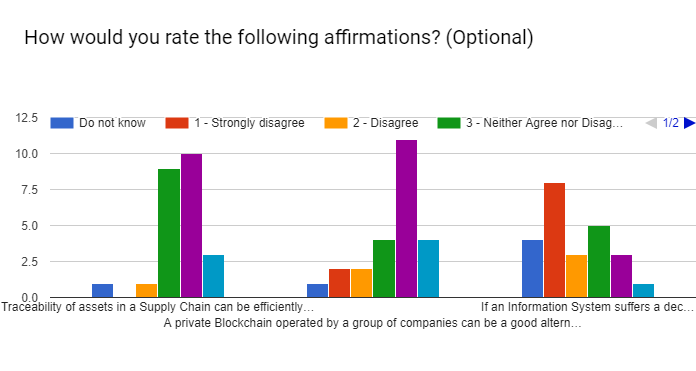
\includegraphics[scale=0.60]{media/affirmations_SC_info_systems.png}
\caption["Rate the affirmations about the use of information systems."]{"Rate the affirmations about the use of information systems."}
\label{fig:affirmations_SC_info_systems}
\end{figure}

%%%%%% TABLE BEGIN %%%%%%%%%%%%%%%%

\begin{table}[h]
\centering
\caption{My caption}
\label{my-label}
\begin{tabular}{l|c|c|c|c|c|c|}
\cline{2-7}
                                                                                                                                        & \multicolumn{1}{l|}{Mode} & \multicolumn{1}{l|}{Median} & \multicolumn{1}{l|}{Mean} & \multicolumn{1}{l|}{\begin{tabular}[c]{@{}l@{}}Standard\\  Deviation\end{tabular}} & \multicolumn{1}{l|}{Range} & \multicolumn{1}{l|}{Skewness} \\ \hline
\multicolumn{1}{|l|}{\begin{tabular}[c]{@{}l@{}}Afirmation 1 - Traceability\\ is already achievable without\\ blockchain.\end{tabular}} & 4                         & 4                           & 3,6522                    & 0,7751                                                                             & 3                          & 0,0812                        \\ \hline
\multicolumn{1}{|l|}{\begin{tabular}[c]{@{}l@{}}Afirmation 2 - Private\\ blockchain as alternative\\ to the cloud.\end{tabular}}        & 4                         & 4                           & 3,5652                    & 1,1610                                                                             & 4                          & -0,9364                       \\ \hline
\multicolumn{1}{|l|}{\begin{tabular}[c]{@{}l@{}}Afirmation 3 - Trade\\ processing speed for security\\ and integration.\end{tabular}}   & 1                         & 2                           & 2,300                     & 1,3018                                                                             & 4                          & 0,4898                        \\ \hline
\end{tabular}
\end{table}

%%%%%% TABLE END %%%%%%%%%%%%%%%%%

\subsection*{4 - Blockchain adoption expectations for the supply chain and Impact of the GDPR on Blockchain}
 
(Placeholder image. Should i divide it in more images?)

\begin{figure}[ht]
    %\makebox[2pt]{}

	\resfig{blockchain_regulate_sc}{Supply chain expectations for Blockchain}
    \resfig{gdpr_blockchain}{Does GDPR limit the use of Blockchain?}
    
      \caption{Blockchain expectation for adoption in supply chain and impact of GDPR on this application.}
    \label{fig:group4_graphics}
\end{figure}


\subsection*{Conclusions from Group 4}